
\documentclass[a4paper]{article}

\usepackage[a4paper, top=8mm, bottom=8mm, left=8mm, right=8mm]{geometry}

\usepackage{polyglossia}
\setdefaultlanguage[babelshorthands=true]{russian}
\setotherlanguage{english}

\usepackage{fontspec}
\setmainfont{FreeSerif}
\newfontfamily{\russianfonttt}[Scale=0.7]{DejaVuSansMono}

\usepackage[tiny, compact]{titlesec}

\usepackage{titling}
\setlength{\droptitle}{-1cm}
\pretitle{\begin{center}\begin{bfseries}\Large}
\posttitle{\par\end{bfseries}\end{center}}
\preauthor{\begin{center}\normalsize}
\postauthor{\par\end{center}\vspace{-1.8cm}}

\usepackage{hyperref}
\usepackage{bookmark}
\usepackage{csquotes}
\usepackage{amsmath}
\usepackage{graphicx}

\title{Реализация свёртки изображений на Python}

\author{Федотов Дмитрий Алексеевич}

\date{}

\begin{document}

\maketitle

\begin{flushright}
    Группа: \emph{\enquote{25.Б41-мм}}

    Кафедра: \emph{системного программирования}

    Научный руководитель: \emph{Пономарев Николай Алексеевич}

    Номер семестра практики: \emph{2}
\end{flushright}

\section{Постановка задачи}

Свёртка является одной из базовых операций цифровой обработки изображений: с её помощью выполняются размытие, повышение резкости и выделение границ. В готовых библиотеках эта операция обычно скрыта за высокоуровневыми функциями, поэтому для понимания алгоритма полезно реализовать её самостоятельно и сравнить результат с промышленными решениями.

Работа выполнялась в рамках учебного проекта по цифровой обработке изображений. \textbf{Целью работы является} разработка собственной реализации операции свёртки изображений на языке Python, а также проверка корректности реализации и сравнение её производительности с готовыми библиотечными решениями.

Результаты работы полезны как учебная реализация базового алгоритма компьютерного зрения: проект позволяет явно увидеть, как ядро свёртки применяется к пикселям изображения, как обрабатываются граничные пиксели и почему специализированные библиотеки оказываются быстрее собственной реализации.

Для достижения цели были поставлены следующие задачи:
\begin{enumerate}
    \item реализовать свёртку для изображений в оттенках серого и цветных изображений в модели RGB;
    \item поддержать ядра размера \(3 \times 3\) и \(5 \times 5\);
    \item реализовать режимы обработки краёв \texttt{reflect}, \texttt{replicate} и \texttt{wrap};
    \item добавить набор ядер для размытия, повышения резкости и выделения границ;
    \item реализовать интерфейс командной строки для выбора изображения, фильтра, режима обработки края и цветового режима;
    \item проверить корректность реализации тестами и провести экспериментальное сравнение производительности с OpenCV и Pillow.
\end{enumerate}

\section{Описание предлагаемого решения}

Свёртка изображения описывается формулой
\[
    C[i,j] = \sum_{k=-p}^{p}\sum_{l=-p}^{p} A[i+k,j+l]B[p+k,p+l],
\]
где \(A\) --- исходное изображение, \(B\) --- ядро размера \((2p+1) \times (2p+1)\), а \(C\) --- результат фильтрации.

Реализация выполнена на Python с использованием NumPy и Pillow. NumPy применяется для представления изображений в виде массивов и для векторизованных вычислений, Pillow --- для чтения изображений и преобразования результата обратно в изображение. В проекте также используется библиотека \texttt{pytest} для функциональных тестов и библиотека \texttt{pytest-benchmark} для измерения производительности.

Основная функция \texttt{convolution} принимает изображение, ядро свёртки и функцию обработки индексов за пределами изображения. Внутри реализации используется единый алгоритм для одноканальных изображений (изображений в оттенках серого) и RGB-изображений. Для этого при обработке изображения в оттенках серого временно добавляется канал, после чего каждый пиксель обрабатывается по общему правилу для всех каналов. После вычисления результат ограничивается диапазоном \([0, 255]\) и приводится к типу \texttt{uint8}.

В проекте реализованы следующие группы ядер:
\begin{itemize}
    \item размытие: \texttt{box\_blur}, \texttt{gaussian\_blur};
    \item выделение границ: \texttt{sobel\_x}, \texttt{prewitt\_y}, \texttt{laplacian}, \texttt{sobel\_x\_5}, \texttt{sobel\_y\_5}, \texttt{laplacian\_5};
    \item повышение резкости: \texttt{sharpen}, \texttt{sharpen\_5}.
\end{itemize}

Например, для этих групп используются следующие ядра:
\begin{align*}
\texttt{box\_blur} &= \frac{1}{9} \begin{bmatrix}1 & 1 & 1 \\ 1 & 1 & 1 \\ 1 & 1 & 1\end{bmatrix},\\
\texttt{sobel\_x} &= \begin{bmatrix}-1 & 0 & 1 \\ -2 & 0 & 2 \\ -1 & 0 & 1\end{bmatrix},\\
\texttt{sharpen} &= \begin{bmatrix}0 & -1 & 0 \\ -1 & 5 & -1 \\ 0 & -1 & 0\end{bmatrix}.
\end{align*}

Для обработки краёв изображения реализованы три режима. Режим \texttt{reflect} отражает координату относительно края, \texttt{replicate} использует ближайший допустимый пиксель, а \texttt{wrap} циклически переносит индекс на противоположную сторону изображения.

\section{Тестирование}

Корректность реализации проверялась тестами с эталонными изображениями, предварительно полученными с помощью библиотеки Pillow и сохранёнными в каталоге \texttt{tests/reference}. Для каждого ядра тест загружает соответствующий файл \texttt{<kernel\_name>.png} и сравнивает его с результатом собственной функции свёртки на одном и том же входном изображении. Поскольку Pillow не предоставляет явного выбора режима обработки краёв для используемой операции фильтрации, сравнение выполняется по внутренней области изображения без краевой рамки шириной в половину размера ядра. Это позволяет проверить основное вычисление свёртки независимо от различий в приграничных пикселях.

\section{Экспериментальное сравнение производительности}

Производительность измерялась с помощью библиотеки \texttt{pytest-benchmark}. В эксперименте сравнивались три реализации: собственная реализация, OpenCV \texttt{cv2.filter2D} и фильтрация через Pillow. Измерения выполнялись на компьютере Apple MacBook Air с процессором Apple M1, 8 ГБ оперативной памяти и операционной системой macOS 15.7.4. Входные данные представляли собой случайно сгенерированные массивы пикселей; такой выбор позволяет сравнивать скорость вычисления свёртки без влияния содержимого конкретного изображения и без затрат на чтение файлов с диска. Проверялись изображения размеров \(128 \times 128\), \(256 \times 256\), \(512 \times 512\), \(1024 \times 1024\), \(1920 \times 1080\), \(2560 \times 1440\), \(3840 \times 2160\) для режима оттенков серого и цветного режима RGB.

В выборочных результатах экспериментального сравнения производительности указывались среднее время и стандартное отклонение. Пример результатов для изображения \(512 \times 512\), режима \texttt{reflect} и ядра \texttt{box\_blur} приведён в таблице~\ref{tab:benchmark-sample}. Сводное сравнение времени выполнения приведено на рисунке~\ref{fig:benchmark-bar}.

\begin{table}[htbp]
    \centering
    \caption{Выборочные результаты измерения времени выполнения, мс}
    \label{tab:benchmark-sample}
    \begin{tabular}{|l|c|c|}
        \hline
        Реализация & Оттенки серого & RGB \\
        \hline
        Собственная реализация & \(41.33 \pm 0.58\) & \(96.64 \pm 1.25\) \\
        OpenCV & \(0.210 \pm 0.005\) & \(0.598 \pm 0.011\) \\
        Pillow & \(0.751 \pm 0.034\) & \(2.75 \pm 0.06\) \\
        \hline
    \end{tabular}
\end{table}

\begin{figure}[htbp]
    \centering
    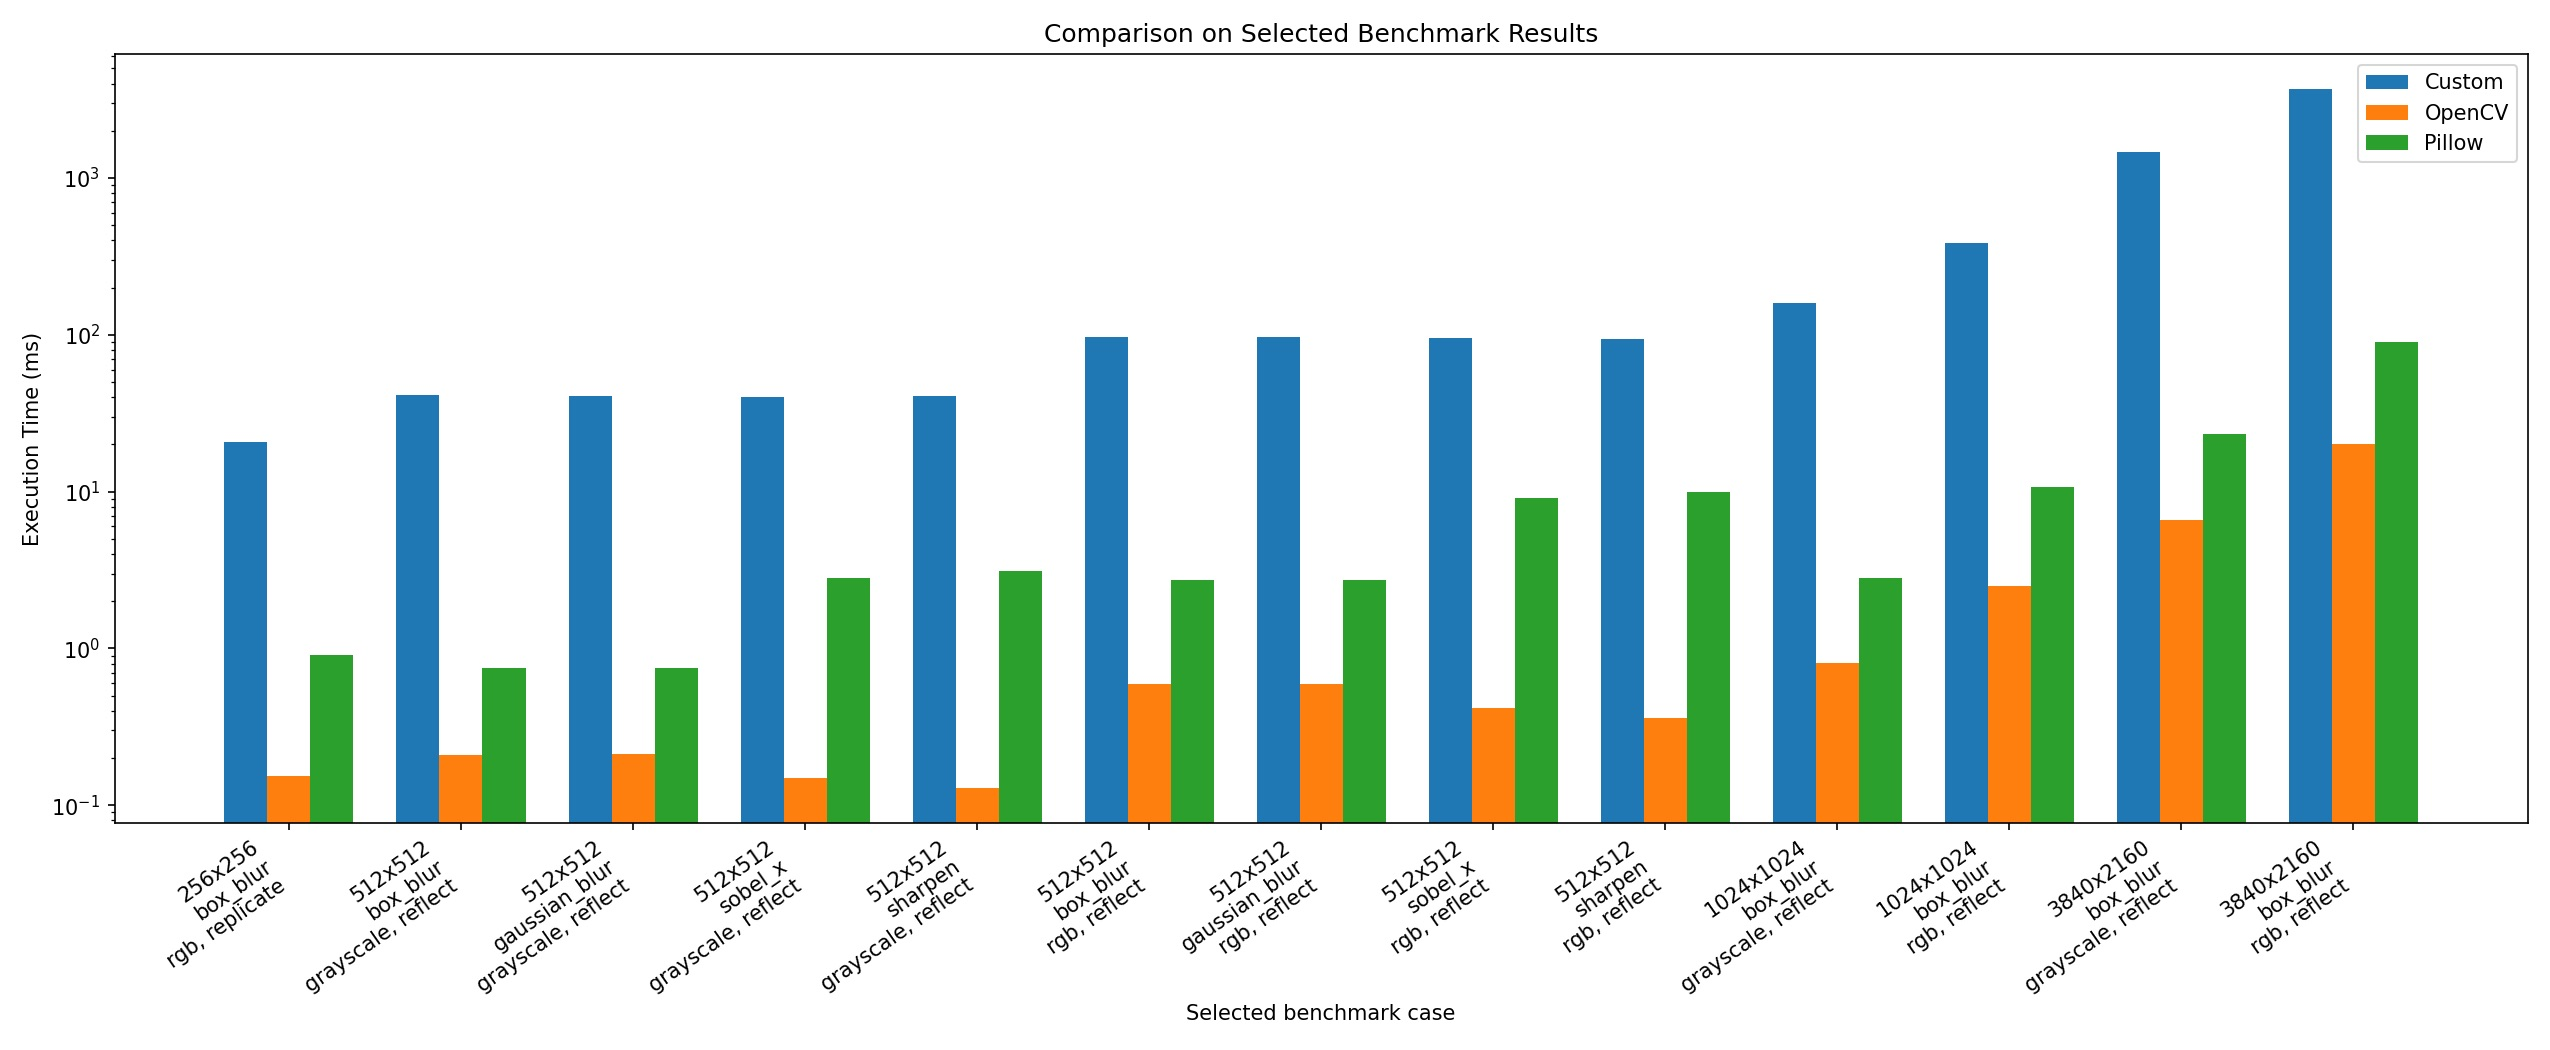
\includegraphics[width=0.82\textwidth]{benchmark_bar.pdf}
    \caption{Сравнение времени выполнения собственной реализации, OpenCV и Pillow}
    \label{fig:benchmark-bar}
\end{figure}

По результатам экспериментов OpenCV оказался быстрее собственной реализации в среднем примерно в 188 раз, а Pillow --- примерно в 23 раза. При этом собственная реализация масштабируется предсказуемо: при увеличении количества пикселей время работы растёт близко к линейной зависимости от размера изображения.

\section{Заключение}

В ходе выполнения работы получены следующие результаты:

\begin{itemize}
    \item реализована операция свёртки изображений на Python с поддержкой изображений в оттенках серого и цветных изображений в модели RGB;
    \item реализованы ядра для размытия, повышения резкости и выделения границ;
    \item реализованы режимы обработки краёв \texttt{reflect}, \texttt{replicate} и \texttt{wrap};
    \item добавлен интерфейс командной строки для выбора входного изображения, фильтра и параметров обработки;
    \item подготовлены тесты корректности по эталонным изображениям;
    \item проведено экспериментальное сравнение производительности собственной реализации с OpenCV и Pillow.
\end{itemize}

Репозиторий: \url{https://github.com/Fedotov-Dmitriy/image-convultion-2sem}.

Техническая документация представлена в файле README репозитория и в файле с анализом результатов экспериментального сравнения производительности \texttt{benchmark\_analysis.md}.

\end{document}
